\documentclass[12pt]{article}
\usepackage[left=1cm, right=1cm, top=2cm,bottom=1.5cm]{geometry} 

\usepackage[parfill]{parskip}
\usepackage[utf8]{inputenc}
\usepackage[T2A]{fontenc}
\usepackage[russian]{babel}
\usepackage{enumitem}
\usepackage[normalem]{ulem}
\usepackage{amsfonts, amsmath, amsthm, amssymb, mathtools}

\usepackage{tabularx}
\usepackage{hhline}

\usepackage{accents}
\usepackage{fancyhdr}
\pagestyle{fancy}
\renewcommand{\headrulewidth}{1.5pt}
\renewcommand{\footrulewidth}{1pt}

\usepackage{graphicx}
\usepackage[figurename=Рис.]{caption}
\usepackage{subcaption}
\usepackage{float}

%%Наименование папки откуда забирать изображения
\graphicspath{ {./images/} }

%%Изменение формата для ввода доказательства
\renewcommand{\proofname}{$\square$  \nopunct}
\renewcommand\qedsymbol{$\blacksquare$}

%%Изменение отступа на таблицах
\addto\captionsrussian{%
	\renewcommand{\proofname}{$\square$ \nopunct}%
}
%% Римские цифры
\newcommand{\RN}[1]{%
	\textup{\uppercase\expandafter{\romannumeral#1}}%
}

%% Для удобства записи
\newcommand{\MR}{\mathbb{R}}
\newcommand{\MC}{\mathbb{C}}
\newcommand{\MQ}{\mathbb{Q}}
\newcommand{\MN}{\mathbb{N}}
\newcommand{\MZ}{\mathbb{Z}}
\newcommand{\MTB}{\mathbb{T}}
\newcommand{\MTI}{\mathbb{I}}
\newcommand{\MI}{\mathrm{I}}
\newcommand{\MJ}{\mathrm{J}}
\newcommand{\MH}{\mathrm{H}}
\newcommand{\MT}{\mathrm{T}}
\newcommand{\MU}{\mathcal{U}}
\newcommand{\MV}{\mathcal{V}}
\newcommand{\MB}{\mathcal{B}}
\newcommand{\MF}{\mathcal{F}}
\newcommand{\MW}{\mathcal{W}}
\newcommand{\ML}{\mathcal{L}}
\newcommand{\MP}{\mathcal{P}}
\newcommand{\VN}{\varnothing}
\newcommand{\VE}{\varepsilon}

\theoremstyle{definition}
\newtheorem{defn}{Опр:}
\newtheorem{rem}{Rm:}
\newtheorem{prop}{Утв.}
\newtheorem{exrc}{Упр.}
\newtheorem{lemma}{Лемма}
\newtheorem{theorem}{Теорема}
\newtheorem{corollary}{Следствие}

\newenvironment{cusdefn}[1]
{\renewcommand\thedefn{#1}\defn}
{\enddefn}

\DeclareRobustCommand{\divby}{%
	\mathrel{\text{\vbox{\baselineskip.65ex\lineskiplimit0pt\hbox{.}\hbox{.}\hbox{.}}}}%
}
%Короткий минус
\DeclareMathSymbol{\SMN}{\mathbin}{AMSa}{"39}
%Длинная шапка
\newcommand{\overbar}[1]{\mkern 1.5mu\overline{\mkern-1.5mu#1\mkern-1.5mu}\mkern 1.5mu}
%Функция знака
\DeclareMathOperator{\sgn}{sgn}

%Функция ранга
\DeclareMathOperator{\rk}{\text{rk}}

%Обозначение константы
\DeclareMathOperator{\const}{\text{const}}

\DeclareMathOperator*{\dsum}{\displaystyle\sum}
\newcommand{\ddsum}[2]{\displaystyle\sum\limits_{#1}^{#2}}

%Интеграл в большом формате
\DeclareMathOperator{\dint}{\displaystyle\int}
\newcommand{\ddint}[2]{\displaystyle\int\limits_{#1}^{#2}}
\newcommand{\ssum}[1]{\displaystyle \sum\limits_{n=1}^{\infty}{#1}_n}

\newcommand{\smallerrel}[1]{\mathrel{\mathpalette\smallerrelaux{#1}}}
\newcommand{\smallerrelaux}[2]{\raisebox{.1ex}{\scalebox{.75}{$#1#2$}}}

\newcommand{\smallin}{\smallerrel{\in}}
\newcommand{\smallnotin}{\smallerrel{\notin}}

\newcommand*{\medcap}{\mathbin{\scalebox{1.25}{\ensuremath{\cap}}}}%
\newcommand*{\medcup}{\mathbin{\scalebox{1.25}{\ensuremath{\cup}}}}%

\makeatletter
\newcommand{\vast}{\bBigg@{3.5}}
\newcommand{\Vast}{\bBigg@{5}}
\makeatother

%Промежуточное значение для sup\inf, поскольку они имеют разную высоту
\newcommand{\newsup}{\mathop{\smash{\mathrm{sup}}}}
\newcommand{\newinf}{\mathop{\mathrm{inf}\vphantom{\mathrm{sup}}}}

%Скалярное произведение
\newcommand{\inner}[2]{\left\langle #1, #2 \right\rangle }

%Подпись символов снизу
\newcommand{\ubar}[1]{\underaccent{\bar}{#1}}

%% Шапка для букв сверху
\newcommand{\wte}[1]{\widetilde{#1}}
\newcommand{\wht}[1]{\widehat{#1}}

%%Трансформация Фурье
\newcommand{\fourt}[1]{\mathcal{F}\left(#1\right)}
\newcommand{\ifourt}[1]{\mathcal{F}^{-1}\left(#1\right)}

%%Символ вектора
\newcommand{\vecm}[1]{\overrightarrow{#1\,}}

%%Пространстов матриц
\newcommand{\mat}[2]{Mat_{#1\times #2}}


%%Взятие в скобки, модули и норму
\newcommand{\parfit}[1]{\left( #1 \right)}
\newcommand{\modfit}[1]{\left| #1 \right|}
\newcommand{\sqparfit}[1]{\left\{ #1 \right\}}
\newcommand{\normfit}[1]{\left\| #1 \right\|}

%%Функция для обозначения равномерной сходимости по множеству
\newcommand{\uconv}[1]{\overset{#1}{\rightrightarrows}}
\newcommand{\uconvm}[2]{\overset{#1}{\underset{#2}{\rightrightarrows}}}


%%Функция для обозначения нижнего и верхнего интегралов
\def\upint{\mathchoice%
	{\mkern13mu\overline{\vphantom{\intop}\mkern7mu}\mkern-20mu}%
	{\mkern7mu\overline{\vphantom{\intop}\mkern7mu}\mkern-14mu}%
	{\mkern7mu\overline{\vphantom{\intop}\mkern7mu}\mkern-14mu}%
	{\mkern7mu\overline{\vphantom{\intop}\mkern7mu}\mkern-14mu}%
	\int}
\def\lowint{\mkern3mu\underline{\vphantom{\intop}\mkern7mu}\mkern-10mu\int}


\begin{document}
\lhead{Линейная алгебра и геометрия}
\chead{Тимашев Д.А.}
\rhead{Лекция - 1}

\section*{Список литературы}
\begin{enumerate}[label=\arabic*)]
	\item Э.Б. Винберг. Курс алгебры. Главы 5-8.
	\item А.И. Кострикин, Ю.И. Манин. Линейная алгебра и геометрия.
	\item А.И. Кострикин. Введение в алгебру, Часть $\RN{2}$: Линейная алгебра.
\end{enumerate}

\section*{Векторные пространства}

Пусть $K$ - \uwave{основное поле}. Элементы основного поля будем называть \uwave{скалярами}.

Например: $K = \MR, \, \MC,\, \MQ, \, \MZ_p$ ($p$ - простое). Первые три это числовые поля, а последнее - не числовое, именно поэтому мы будем называть элементы поля скалярами, а не числами.

\begin{defn}
	\uwave{Векторное (линейное) пространство} над полем $K$ - это множество $V$, элементы которого называются \uwave{векторами}, на котором заданы две операции:
	\begin{enumerate}[label=\arabic*)]
		\item \uline{Сложение векторов}: $V \times V \to V, \, (u,v) \mapsto w = u + v$;
		\item \uline{Умножение векторов на скаляры}: $K \times V \to V,\, (\lambda, v) \mapsto w = \lambda {\cdot}v$; 
	\end{enumerate}
	так, что выполняются \uwave{аксиомы векторного пространства}:
	\begin{enumerate}[label=(\arabic*)]
		\item $u + v = v + u, \, \forall u,v \in V$;
		\item $(u + v) + w = u + (v + w), \, \forall u,v,w \in V$;
		\item $\exists \, 0 \in V \colon \forall v \in V, \, v + 0 = v$ (существует \uwave{нулевой вектор}), иногда будем обозначать $\vecm{0}$;
		\item $\forall v \in V, \, \exists \, w \colon v + w = 0$, где $w$ называется \uwave{противоположным вектором} и обозначается $w = -v$;
		\item $\lambda{\cdot}(\mu{\cdot}v) =(\lambda{\cdot}\mu){\cdot}v, \, \forall \lambda, \mu \in K, \, \forall v \in V$;
		\item $\lambda{\cdot}(u + v) = \lambda{\cdot}u + \lambda{\cdot}v, \, \forall \lambda \in K, \, \forall u,v \in V$
		\item $(\lambda + \mu){\cdot}v = \lambda{\cdot}v + \mu{\cdot}v, \, \forall \lambda, \mu \in K, \, \forall v \in V$;
		\item $1 {\cdot}v = v, \, \forall v \in V$;
	\end{enumerate}
\end{defn}
\begin{rem}
	По отношению к операции сложения $V$ образует абелеву группу.
\end{rem}

\subsection*{Примеры векторных пространств}

\begin{enumerate}[label=\arabic*)]
	\item \uwave{Пространство геометрических векторов}: $V = \{\text{геометрические векторы в пространстве}\}$, $K = \MR$.
	
	\textbf{\uline{Вектора}}: направленный отрезок, причем не закрепляем у него начальную точку (свободные векторы). Векторы, полученные параллельным переносом считаем одинаковыми. 
	
	\textbf{\uline{Операции}}:
	\begin{enumerate}
		\item[($+$):] Правило параллелограмма: вектора откладываются от одного и того же начала, строим на них параллелограмм и берем вектор идущий по диагонали этого параллелограмма;
		\item[($\, \cdot\, $):] Соответствующий отрезок растягиваем или сжимаем в нужное число раз. Если коэффициент отрицательный $\Rightarrow$ меняем направление. Если коэффициент нулевой $\Rightarrow$ получаем нулевой вектор (вектор у которого начало и конец совпадают);
	\end{enumerate}
	
	\begin{figure}[H]
		\centering
		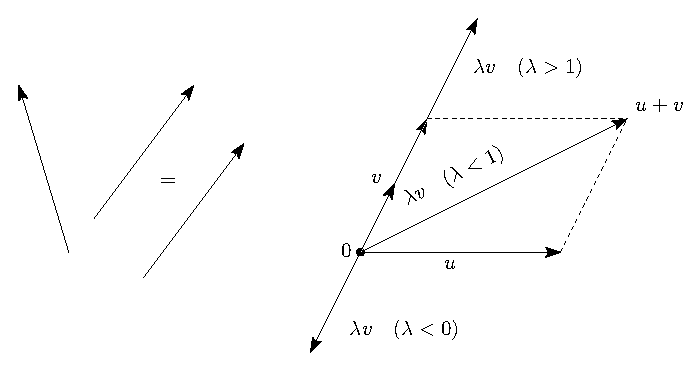
\includegraphics[width=0.5\textwidth]{LAL1_1.eps}
		\label{LAL1_1}
		\caption{Пространство геометрических векторов.}
		\label{fig: Проекция на пространство}
	\end{figure}

	\item \uwave{Арифметическое векторное пространство}: $V = K^n$.
	
	\textbf{\uline{Вектора}}: упорядоченные наборы из $n$ элементов основного поля: $x = (x_1, x_2, \dotsc, x_n), \, \forall i ,\, x_i \in K$.
	
	\textbf{\uline{Операции}}: Определяются покомпонентно:
	\begin{enumerate}
		\item[($+$):] $x + y = (x_1 + y_1, x_2 + y_2, \dotsc, x_n + y_n)$;
		\item[($\, \cdot\, $):] $\lambda{\cdot}x = (\lambda{\cdot}x_1, \lambda{\cdot}x_2, \dotsc, \lambda{\cdot}x_n)$;
	\end{enumerate}

	\item \uwave{Пространство матриц фиксированного размера}: $V = \mat{m}{n}(K)$ - можно отождествить с $K^{m{\cdot}n}$. Операции с матрицами мы рассматривали ранее в курсе алгебры.
	\begin{rem}
		Матрицу всегда можно разложить в одну длинную строку: длиной $mn$.
	\end{rem}

	\item \uwave{Пространство функций}: $V =  \MF(X,K) = \{f \colon X \to K\}$.
	
	\textbf{\uline{Операции}}: 
	\begin{enumerate}
		\item[($+$):] $\forall f,g \in \MF(X,K), \, f + g \in \MF(X,K) \colon (f+g)(x) = f(x) + g(x), \, \forall x \in X$;
		\item[($\, \cdot\, $):] $\forall f \in \MF(X,K), \, \forall \lambda \in K, \, \lambda{\cdot}f \in \MF(X,K) \colon (\lambda{\cdot}f)(x) = \lambda{\cdot}f(x), \, \forall x \in X$;
	\end{enumerate}
	
	\item \uwave{Пространство многочленов от переменной} $t$: $V = K[t]$. Многочлены можно складывать, умножать на элементы поля снова будем получать многочлены $\Rightarrow$ определены операции.
	\textbf{\uline{Операции}}: 
	\begin{enumerate}
		\item[($+$):] $\forall P(x),Q(x) \in K[t], \, P(x) + Q(x) \in K[t]$;
		\item[($\, \cdot\, $):] $\forall P(x) \in K[t], \, \forall \lambda \in K, \, \lambda{\cdot}P(x) \in K[t]$;
	\end{enumerate}
	
	
	\item \uwave{Расширение полей}: пусть $L$ - поле, $K \subseteq L$ - подполе, сложение умножение определены по определению поля, в частности, элементы поля $L$ можно складывать между собой и умножать на элементы подполя $K \Rightarrow V = L$ - векторное пространство над $K$. Например, $\MR \supset \MQ$, $\MC \supset \MR$.	
\end{enumerate}

\newpage
\subsection*{Свойства векторов и операций над ними}

\begin{corollary}
	Нулевой вектор единственен.
\end{corollary}
\begin{proof}
	Пусть $0_1$ и $0_2$ - два нулевых вектора, сложим их: 
	$$
		0_1 = 0_1 + 0_2 = 0_2 \Rightarrow 0_1 = 0_2
	$$
	где $0_1 + 0_2 = 0_2$, так как $0_1$ - нулевой вектор и $0_1 + 0_2 = 0_1$, так как $0_2$ - нулевой вектор.
\end{proof}

\begin{corollary}
	У каждого вектора $\exists!$ противоположный вектор.
\end{corollary}
\begin{proof}
	Пусть есть два противоположных вектора $w_1 \in V$ и $w_2 \in V$ вектору $v \in V$. Сложим их все и расставим скобки:
	$$
		w_1 + 0 = w_1 + (v+ w_2) = (w_1 + v) + w_2 = 0 + w_2 = w_2 \Rightarrow w_1 = w_2
	$$
\end{proof}

\begin{corollary}
	$\forall \lambda \in K, \, \lambda {\cdot}\vecm{0} = \vecm{0}$.
\end{corollary}
\begin{proof}
	$$
		\lambda{\cdot}\vecm{0} = \lambda{\cdot}\left(\vecm{0} + \vecm{0}\right) = \lambda{\cdot}\vecm{0} + \lambda{\cdot}\vecm{0} \Rightarrow +\left(-\lambda{\cdot}\vecm{0}\right) \Rightarrow \vecm{0} = \lambda{\cdot}\vecm{0} + \vecm{0} = \lambda{\cdot}\vecm{0}
	$$
\end{proof}
\begin{corollary}
	$\forall v \in V, \, 0{\cdot}v = \vecm{0}$.
\end{corollary}
\begin{proof}
	$$
		0{\cdot}v = (0 + 0){\cdot}v = 0{\cdot}v + 0{\cdot}v \Rightarrow +(-0{\cdot}v) \Rightarrow +\left(-0{\cdot}v\right) \Rightarrow \vecm{0} = 0{\cdot}v + \vecm{0} = 0{\cdot}v
	$$
\end{proof}

\begin{corollary}
	$\forall v \in V, \, (-1){\cdot}v = - v$.
\end{corollary}
\begin{proof}
	Рассмотрим сумму:
	$$
		v + (-1){\cdot}v = 1{\cdot}v + (-1){\cdot}v = (1 + (-1)){\cdot}v = 0{\cdot}v = \vecm{0} \Rightarrow (-1){\cdot}v = - v
	$$
\end{proof}
\begin{rem}
	Запись скалярного множителя слева или справа - не важно, потому что множители имеют разные типы. Иногда бывает удобно записывать умножение на скаляры справа:
	$$
		\forall v \in V, \, \forall \lambda \in V, \, v{\cdot}\lambda \coloneqq \lambda{\cdot}v
	$$
	В дальнейшем увидим, что это может быть достаточно удобно. При этом сохраняется вид аксиом векторного пространства, например, ассоциативность (воспользуемся коммутативностью умножения поля):
	$$
		(v{\cdot}\lambda){\cdot}\mu = \mu{\cdot}(\lambda{\cdot} v) = (\mu {\cdot}\lambda){\cdot}v = (\lambda{\cdot}\mu){\cdot}v = v{\cdot}(\lambda{\cdot}\mu)
	$$
	Остальные аксиомы сохраняются тем более.
\end{rem}
\newpage

\subsection*{Линейная зависимость}
\begin{defn}
	\uwave{Линейная комбинация} векторов $v_1,\dotsc, v_m \in V$ с коэффициентами $\lambda_1, \dotsc, \lambda_m \in K$ - это конечная сумма вида:
	$$
		\lambda_1 {\cdot}v_1 + \lambda_2{\cdot} v_2 + \dotsc + \lambda_m{\cdot}v_m
	$$
\end{defn}
\begin{defn}
	Линейная комбинация называется \uwave{тривиальной}, если: $\lambda_1 = \lambda_2 = \dotsc = \lambda_m = 0$.
\end{defn}

\begin{defn}
	Система векторов $S = (v_1, \dotsc v_m)$ называется \uwave{линейно зависимой}, если $\exists$ нетривиальная (то есть $\exists \, \lambda_i \neq 0$) линейная комбинация векторов этой системы равная нулю:
	$$
		\lambda_1 v_1 + \dotsc + \lambda_m v_m = 0
	$$
	В противном случае, она называется \uwave{линейно независимой}.
\end{defn}
\begin{theorem}(\textbf{основная лемма о линейной зависимости})
	Пусть у нас есть две системы векторов: 
	$$
		S = (v_1, \dotsc, v_m), \quad T = (w_1,\dotsc, w_n)
	$$
	причём $\forall v_i \in S$ является линейной комбинацией векторов из $T$ и $m > n \Rightarrow S$ - линейно зависима.
\end{theorem}
\begin{rem}
	Можно переформулировать теорему следующим образом: если $S$ линейно независима и линейно выражается через $T$, то $m \leq n$.
\end{rem}
\begin{proof}
	Доказывается в курсе алгебры первого семестра.
\end{proof}

\begin{defn}
	Будем говорить, что система векторов $S$ \uwave{порождает} векторное пространство $V$, если:
	$$
		\forall v \in V, \, \exists \, v_1,\dotsc, v_n \in S, \, \exists \, \lambda_1, \dotsc, \lambda_n \in K \colon v = \lambda_1 v_1 + \dotsc + \lambda_n v_n
	$$
\end{defn}

\begin{prop}
	Пусть $S = (v_1,\dotsc, v_n)$ - конечная система векторов, тогда следующие условия эквивалентны:
	\begin{enumerate}[label=(\arabic*)]
		\item $S$ - линейно независима и порождает $V$;
		\item $S$ - является максимальной линейно независимой системой векторов в $V$
	\end{enumerate}
\end{prop}
\begin{defn}
	Система векторов называется \uwave{максимальной}, если при добавлении к ней хотя бы одного вектора система становится линейно зависимой.
\end{defn}
\begin{proof}
	\hfill\\
	$(1) \Rightarrow (2)$ $\forall v \in V$ в силу линейной независимости верно:
	$$
		v = \lambda_1 v_1 + \dotsc + \lambda_n v_n \Rightarrow \lambda_1 v_1 + 	\dotsc + \lambda_n v_n + (-1)v = 0, \, (-1) \neq 0
	$$ 
	Cистема нетривиальна $\Rightarrow S \cup \{v\}$ - линейно зависима $\Rightarrow S$ - максимальная линейно независимая.
	
	$(2) \Rightarrow (1)$ $\forall v \in V, \, S = (v_1,\dotsc,v_n, v)$ - линейно зависима, тогда:
	$$
		\exists \, \mu_i \neq 0 \colon \mu_1 v_1 + \dotsc + \mu_n v_n + \mu_{n+1} v = 0 \Rightarrow \mu_{n+1} \neq 0
	$$
	Если $\mu_{n+1} = 0$, то мы бы получили, что система $S$ - линейна зависима, а это не так. Тогда:
	$$
		v = \left(-\dfrac{\mu_1}{\mu_{n+1}}\right){\cdot}v_1  + \dotsc + \left(-\dfrac{\mu_n}{\mu_{n+1}}\right){\cdot}v_n	
	$$
	Получили, что вектор $v \in V$ выражается через векторы системы $S \Rightarrow S$ пораждает пространство $V$.
\end{proof}

\begin{defn}
	Упорядоченная система векторов, удовлетворяющих эквивалентным условиям $(1)$ и $(2)$ из утверждения $1$ называется \uwave{базисом пространства} $V$. Стандартное обозначение базиса: 
	$$
		e = (e_1, \dotsc, e_n)
	$$
\end{defn}

\begin{rem}
	Также заметим, что мы работаем с конечными базисами, чтобы не разбираться с некоторыми теоретико-множественными трудностями бесконечномерных пространств. Далее ещё это обговорим.
\end{rem}

\begin{prop}
	$\forall x \in V, \, \exists!$ разложение $x = x_1{\cdot}e_1 + \dotsc x_n{\cdot}e_n, \, x_i \in K$ по базису $e$.
\end{prop}
\begin{proof}\hfill\\
	\textbf{\uline{Существование}}: Поскольку базис это порождающая система векторов, то $\forall x \in V$ можно разложить в виде линейной комбинации базисных векторов: $\exists\, x_1, \dotsc, x_n \in K \colon x = x_1e_1 + \dotsc + x_ne_n$.
	
	\textbf{\uline{Единственность}}: Пусть $\exists$ другое разложение $x = x_1'{\cdot}e_1 + \dotsc + x_n'{\cdot}e_n$, следовательно вычтем одно разложение из другого:
	$$
		(x_1 - x_1'){\cdot}e_1 + \dotsc + (x_n - x_n'){\cdot}e_n = 0 \Rightarrow x_1 - x_1' = \dotsc =  x_n - x_n' = 0 \Rightarrow \forall i = \overline{1, n}, \, x_i = x_i'
	$$
	где мы воспользовались определением базиса (вектора линейно независимы $\Rightarrow$ равенство их линейной комбинации нулю возможно только в тривиальном случае).
\end{proof}

\begin{defn}
	\uwave{Координатами вектора} $x$ в базисе $e$ называются $x_i \in K$ из его разложения $x = x_1{\cdot}e_1 + \dotsc x_n{\cdot}e_n$.
\end{defn}
В дальнейшем удобно будет записывать разложение по базису в матричном виде:
$$
	x = \begin{pmatrix}
		e_1 & \dotsc & e_n
	\end{pmatrix}{\cdot}
	\begin{pmatrix}
		x_1 \\
		\vdots\\
		x_n
	\end{pmatrix} = e{\cdot}X
$$
где $X$ - столбец координат вектора $x$ в базисе $e$.

\begin{prop}
	Во всех базисах пространства $V$ одинаковое количество векторов.
\end{prop}
\begin{proof}
	Следует сразу из основной леммы о линейной зависимости: если бы было разное число, то тот базис, в котором векторов было бы больше он бы линейно выражался через тот базис, в котором векторов было бы меньше $\Rightarrow$ базис в котором больше векторов был бы линейно зависим $\Rightarrow$ противоречие.
\end{proof}

\begin{defn}
	\uwave{Размерностью} векторного пространства $V$ называется количество векторов в любом базисе этого пространства. \textbf{\uline{Обозначение}}: $\dim{V}$.
\end{defn}

\subsection*{Примеры базисов векторных пространств}

\begin{enumerate}[label=(\arabic*)]
	\item Арифметическое пространство: $K^n$. 
	
	\textbf{\uline{Стандартный базис}}: $
		\begin{pmatrix}
			e_1 & \dotsc & e_n
		\end{pmatrix}$, где $\forall i = \overline{1,n}, \, e_i = \underset{
		\begin{matrix}
			&&&i&&&
		\end{matrix}}{
		\begin{pmatrix}
			0 & \dotsc & 0 & 1 & 0 & \dotsc & 0 
		\end{pmatrix}}$.
	
	$\forall x = \begin{pmatrix}
		x_1 & \dotsc & x_n
	\end{pmatrix} \in K^n, \, x = x_1{\cdot}e_1 + \dotsc + x_n{\cdot}e_n$, где $x_i$ - координаты в стандартном базисе;
	\item Пространство матриц: $\mat{m}{n}(K)$. 
	
	\textbf{\uline{Стандартный базис}}: $E_{ij} = 
	\begin{matrix}
		\\
		\\
		i\\
		\\
		\\
	\end{matrix}\,
	\underset{
	\begin{matrix}
		&&j&&
	\end{matrix}
	}{
	\begin{pmatrix}
		0 & \dotsc & 0 & \dotsc & 0\\
		\vdots & \ddots & \vdots & \ddots & \vdots \\
		0 & \dotsc & 1 & \dotsc & 0 \\
		\vdots & \ddots & \vdots & \ddots & \vdots \\
		0 & \dotsc & 0 & \dotsc & 0
	\end{pmatrix}
	}$ - \uwave{матричные единицы}.

	$\forall A \in \mat{m}{n}(K), \, A = \ddsum{\substack{i = 1,\dotsc,m\\j = 1,\dotsc, n}}{} a_{ij}E_{ij} = \ddsum{i = 1}{m}\ddsum{j = 1}{n}a_{ij}E_{ij}$, где $a_{ij}$ - элементы матрицы $A$;
	
	\item Поле комплексных чисел над полем вещественных чисел: $\MC \supset \MR$.
	
	\textbf{\uline{Базис}}: $(1,i)$, то что это базис (существует и единственное разложение по базису) - свойство алгебраической формы записи комплексного числа.
	
	$\forall z \in \MC, \, z = x + iy, \, x = \operatorname{Re}(z) \in \MR, \, y = \operatorname{Im}(z) \in \MR$.
	\begin{figure}[H]
		\centering
		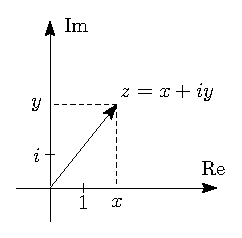
\includegraphics[width=0.25\textwidth]{LAL1_2.eps}
		\label{LAL1_2}
		\caption{Поле $\MC$ над  $\MR$.}
		\label{fig: поле компл над веществ}
	\end{figure}

	\item Пространство многочленов: $K[t]$.
	
	Конечный набор одночленов: $1,t,t^2, \dotsc, t^n$ - линейно независимая система векторов при $\forall n$, поскольку две разные комбинации одночленов дают разные многочлены, если линейная комбинация равна $0$, то только в тривиальном случае $\Rightarrow$ есть сколь угодно большая линейно независимая система в заданном пространстве $\Rightarrow$ нет конечного базиса;
\end{enumerate}

\begin{defn}
	Векторное пространство $V$ называется \uwave{конечномерным}, если в нём есть конечный базис и \uwave{бесконечномерным} в противном случае.
\end{defn}
\newpage
\section*{Изоморфизмы векторных пространств}
Бывает так, что разные векторные пространства обладают одинаковыми свойствами с точки зрения линейной алгебры, то есть устроены одинаково.

\begin{defn}
	\uwave{Изоморфизм векторных пространств} это такое отображение $\varphi \colon V \to W$, где $V$ и $W$ - два векторных пространства над одним и тем же полем $K$, которое удовлетворяет двум свойствам:
	\begin{enumerate}[label=\arabic*)]
		\item $\varphi$ - биективно;
		\item $\varphi$ - согласовано с операциями: 
		$$
			\varphi(x + y) = \varphi(x) + \varphi(y), \, \forall x,y \in V
		$$
		$$
			\varphi(\lambda{\cdot}x) = \lambda{\cdot}\varphi(x), \, \forall \lambda \in K, \, \forall x \in V
		$$	
	\end{enumerate}
	\textbf{\uline{Обозначение}}: $\varphi \colon V \xrightarrow[]{\sim} W$ или $\varphi \colon V \xrightarrow[\sim]{} W$.
\end{defn}
\begin{defn}
	Пространства $V$ и $W$ \uwave{изоморфны}, если $\exists$ изоморфизм $\varphi \colon V \xrightarrow[]{\sim} W$. \textbf{\uline{Обозначение}}: $V \simeq W$.
\end{defn}
Если между пространствами есть изоморфизм, то все свойства линейной алгебры, формулируемые в терминах операций над векторами, если выполнены в одном пространстве, то будут и в другом.

\begin{theorem}
	Любое векторное пространство $V$ над полем $K$, размерности $n < \infty$ изоморфно $K^n$.
\end{theorem}
\begin{proof}
	Выберем базис $e = \begin{pmatrix}
		e_1 & \dotsc & e_n
	\end{pmatrix}$ в пространстве $V$ и построим отображение $\varphi \colon K^n \to V$ следующим образом:
	$$
		\varphi \colon X = \begin{pmatrix}
				x_1 \\
				\vdots\\
				x_n
			\end{pmatrix} \mapsto x = e{\cdot}X
	$$
	Проверим биективность:
	\begin{enumerate}[label=\arabic*)]
		\item \textbf{\uline{Инъективность}}: следует из единственности разложения вектора по базису:
		$$
			\varphi(a) = \varphi(b) \Rightarrow a_1 e_1 + \dotsc + a_n e_n = b_1 e_1 + \dotsc b_n e_n \Rightarrow a = b
		$$
		\item 	\textbf{\uline{Сюръективность}}: также следует из разложения вектора по базису:
		$$
			\forall x \in V, \, \exists \, x_1, \dotsc, x_n \in K \colon x = x_1 e_1 + \dotsc x_n e_n = e{\cdot}x = \varphi(x)
		$$
	\end{enumerate}
	Следовательно, отображение - биективно. Cогласованность с операциями - очевидна:
	$$
		\forall a,b \in K^n, \, \varphi(a + b) = e(a + b) = (a_1 + b_1)e_1 + \dotsc (a_n + b_n)e_n = a_1 e_1 + \dotsc + a_n e_n + b_1 e_1 + \dotsc + b_n e_n =
	$$
	$$
		= ea + eb = \varphi(a) + \varphi(b)
	$$
	$$
		\forall a \in K^n, \, \forall \lambda \in K, \, \varphi(\lambda a) = e(\lambda a) = \lambda a_1 e_1 + \dotsc \lambda a_n e_n = \lambda{\cdot}(a_1 e_1 + \dotsc + a_n e_n) = \lambda \varphi(a)
	$$
	В результате, мы получаем, что отображение это изоморфизм.
\end{proof}

\textbf{\uline{Пример}}: Пространство геометрических векторов (направленных отрезков в пространстве) $V$ имеет размерность $3 \Rightarrow V \simeq \MR^3$.

\end{document}